\documentclass[manuscript,screen,review]{acmart}

\begin{document}

\title{The Name of the Title is Hope}


\author{Ben Trovato}
\authornote{Both authors contributed equally to this research.}
\email{trovato@corporation.com}
\orcid{1234-5678-9012}
\author{G.K.M. Tobin}
\authornotemark[1]
\email{webmaster@marysville-ohio.com}
\affiliation{%
  \institution{Institute for Clarity in Documentation}
  \streetaddress{P.O. Box 1212}
  \city{Dublin}
  \state{Ohio}
  \country{USA}
  \postcode{43017-6221}
}

\author{Lars Th{\o}rv{\"a}ld}
\affiliation{%
  \institution{The Th{\o}rv{\"a}ld Group}
  \streetaddress{1 Th{\o}rv{\"a}ld Circle}
  \city{Hekla}
  \country{Iceland}}
\email{larst@affiliation.org}

\author{Valerie B\'eranger}
\affiliation{%
  \institution{Inria Paris-Rocquencourt}
  \city{Rocquencourt}
  \country{France}
}

\author{Aparna Patel}
\affiliation{%
 \institution{Rajiv Gandhi University}
 \streetaddress{Rono-Hills}
 \city{Doimukh}
 \state{Arunachal Pradesh}
 \country{India}}

\author{Huifen Chan}
\affiliation{%
  \institution{Tsinghua University}
  \streetaddress{30 Shuangqing Rd}
  \city{Haidian Qu}
  \state{Beijing Shi}
  \country{China}}

\author{Charles Palmer}
\affiliation{%
  \institution{Palmer Research Laboratories}
  \streetaddress{8600 Datapoint Drive}
  \city{San Antonio}
  \state{Texas}
  \country{USA}
  \postcode{78229}}
\email{cpalmer@prl.com}

\author{John Smith}
\affiliation{%
  \institution{The Th{\o}rv{\"a}ld Group}
  \streetaddress{1 Th{\o}rv{\"a}ld Circle}
  \city{Hekla}
  \country{Iceland}}
\email{jsmith@affiliation.org}

\author{Julius P. Kumquat}
\affiliation{%
  \institution{The Kumquat Consortium}
  \city{New York}
  \country{USA}}
\email{jpkumquat@consortium.net}


\begin{abstract}
The contemporary landscape of virtual world design is characterized by the ubiquity of diverse tools and terrain design engines, which have significantly reduced the barriers to entry in this domain. Despite this progress, the predominant input modalities of mice and keyboards fail to provide users with haptic feedback during the processes of designing, testing, and experiencing virtual environments. Addressing this limitation, we introduce HaptiEditor, a virtual terrain editing tool that integrates haptic feedback through the utilization of force-feedback capabilities offered by the Haply 2Diy device, implemented within the Unity game engine framework. Our primary objective is to enhance both the design process and the evaluative capacity of designers, as well as to enrich the immersive engagement of users or players navigating these virtual worlds.  
\end{abstract}

\keywords{Haptics, Tool Design, Unity, Haply, ForceFeedback, Haptic Texture Rendering}

\maketitle

\section{Introduction} \label{sec:intro}
%% Describing The problem
Haptics interfaces are often used for enhancing sculpting experiences.
However, no significant implementation of force-feedback interfaces in the case of terrain editing and terrain painting has been created.
Many existing haptic-augmented sculpting applications might be applicable to this task, but use haptic devices with three, or even six degrees of freedom, which are often both large and expensive.
With HaptiEditor, we intend to use the target domain of terrain editing to our advantage, developing a compelling user interface with a relatively inexpensive two degree of freedom device.

%% Describing our solution
HaptiEditor is a Unity application which has for objective to edit maps and terrain by painting textures and objects on different scales. 
By using the Haply 2DIY we hope to create an interesting approach to terrain creation and edition through haptic feedback.
The goal is to allow real time editing of a virtual space, and simultaneously feel the effect of the changes right away.

%% Tell your Story
The development period spaned 3 months during the Winter session of 2024, as part of the cross-institutional CanHap501 course.
CanHap501 is a program which covers multiple Canadian universities, introducing graduate MSc students to haptic interfaces. 
The course teaches students how to conceptualize, prototype, develop and do user evaluation with multimodal human-computer interfaces and haptic experiences.
This project is being developed in a team of three, with each member in different location (Montreal, Okanagan and Vancouver).

%% Justify the approach
Since the development timeline of this project is very short, we decided to go with a rapid prototyping approach; developing features in parallel during the course.
Moreover, since we didn't have enough time to create a fully fledged terrain editor software,
we use Unity to simplify a lot of the designing and implementation to get to experiment with the haptic side of the project quicker.
This choice proved advantageous, as Unity, a game engine, already implements some solid systems for collision, forces and texturing.

%% State your contributions
HaptiEditor allows exploration of terrain at different scales via a novel zooming system.
Using a system of sampling existing textures form the surface's material in order to create haptic feedback and Unity's collision system, HaptiEditor is able to provide different haptic feedback depending on the scale of the end effector scale in the scene.
This allows a haptic continuum to enable the user to feel the terrain they are editing at any scale they would potentially need.

%% Overview of the paper
This report is a statement of the advancements and findings made during the development of HaptiEditor. 
We will go over the different avenues tried in order to create HaptiEditor, what was prototyped and how it shaped the current software. 
We will then examine the results gathered through semiformal user testing and the overall appreciation the project received. 
The results of the user testing and our implementation will thoroughly be discussed in the Discussions section.


\section{Related Work} \label{sec:rel_work}
Lorem ipsum dolor sit amet, consectetur adipiscing elit. Ut accumsan arcu bibendum purus laoreet rutrum. Integer aliquam arcu gravida dignissim vestibulum. Aenean ut congue purus. Nullam eleifend, justo non bibendum efficitur, odio felis porta ligula, semper commodo massa erat vel tellus. Nullam non nibh vel eros imperdiet vestibulum sit amet a ex. Proin mattis dui at tortor ultricies, id pulvinar nisi euismod. Duis sed massa in dui aliquet hendrerit. Praesent aliquam luctus nisi non lobortis. Sed bibendum magna orci, vitae pharetra nibh mattis ac. Mauris quis lacus vitae est posuere blandit. Vestibulum ante ipsum primis in faucibus orci luctus et ultrices posuere cubilia curae; Sed quis augue id lacus egestas tincidunt. Duis et risus vel justo vestibulum feugiat. Donec neque nisl, luctus vitae leo sit amet, vulputate maximus nunc. Cras et velit ut ex ultrices venenatis eget vel odio. Proin fringilla, ante vel fermentum bibendum, ipsum neque dictum dolor, nec semper urna felis sit amet nibh. \cite{klatzky2013haptic}

Fusce eget tristique ante. Proin rutrum est eget semper iaculis. Morbi pulvinar urna non dui dapibus faucibus. Suspendisse tincidunt, sapien non luctus varius, justo ante consectetur erat, quis efficitur ante felis ultricies urna. Sed finibus justo a fringilla finibus. Praesent vitae elit ac nisi maximus tristique. In ac orci volutpat, bibendum quam in, tristique dui. Integer eget nulla id nulla ultricies molestie nec id lacus. Donec eleifend rutrum risus et tempor. Morbi lobortis maximus vestibulum.

Fusce ultrices at sapien tristique semper. Ut congue, ex quis ultrices dictum, nunc ligula ornare sem, in pellentesque felis risus in diam. In hac habitasse platea dictumst. Pellentesque ultricies lectus et congue mattis. Integer a ligula non est dapibus mattis eget ut diam. Sed et ex purus. Aliquam pretium, lacus nec molestie tempus, erat magna mollis tortor, quis pulvinar nulla ipsum eu turpis. Sed nibh erat, posuere in dolor ut, accumsan luctus felis. Nam sit amet elit purus. Nulla rhoncus turpis vitae odio viverra commodo pretium nec libero. Lorem ipsum dolor sit amet, consectetur adipiscing elit. Integer in mi quis odio gravida lacinia. Nam massa mauris, tempor consequat felis id, blandit tincidunt nibh. Integer elementum ex vitae nibh fermentum, ac tincidunt libero semper.


\section{Approach} \label{sec:approach}
This project attempts to deliver on a haptics focused terrain editing experience first and foremost. The overaching approach was to first establish a reliable coupling via a virtual proxy to Unity's physics system, and then create a proof of concept terrain editing tool which is driven by the aforementioned virtual proxy.

The three fundamental questions we had were as follows:

\begin{enumerate}
    \item How would we design a generic virtual coupling between Unity's physics engine and the Haply's force feedback mechanisms?
    \item How would we detect and render textures in realtime?
    \item How would we design the tool itself, with the main mode of interaction being through the Haply?
\end{enumerate}

\subsection{How would we design a generic virtual coupling between Unity's physics engine and the Haply's force feedback mechanisms?}

We initially employed the Unity template obtained from the Haply GitLab repository as the foundation for our implementation. However, upon closer examination, it became evident that the forces applied were hardcoded, prompting us to adopt a \textit{PD controller} model facilitated by a virtual proxy (\textit{See \ref*{fig:virtual-coupling}}), as elaborated below.

In our implementation, we utilized Unity game objects, specifically employing one designated as the "\textbf{End Effector Actual}" to track the ideal positional data of the Haply, and another marked as the "\textbf{End Effector Representation}" equipped with a built-in sphere collider. This was to allow it to interact with Unity's physics engine. Subsequently, we established a \textit{PD controller} relationship between these two entities. The underlying operational logic mandated the "\textbf{End Effector Representation}" to consistently attempt to minimize the euclidean distance between itself and the "\textbf{End Effector Actual}". This behavior was governed primarily by the proportional component of the \textit{PD controller}, supplemented by the derivative component to offer additional smoothing (\textit{See \ref*{fig:virtual-coupling-a}}). In instances where the "\textbf{Representation}" detected any physical collisions, it directed the Haply to exert a force in the direction of the "\textbf{Representation}" from the "\textbf{Actual}" (\textit{See \ref*{fig:virtual-coupling-b}}). This would happen in parallel to the distance minimization attempts of the "\textbf{Representation}". Consequently, this establishment facilitated an adaptable virtual coupling mechanism, subject to the influence of Unity's physics engine via the intermediary proxy.


\begin{figure}[htbp]
    \centering
    \begin{subfigure}[b]{0.4\textwidth}
        \centering
        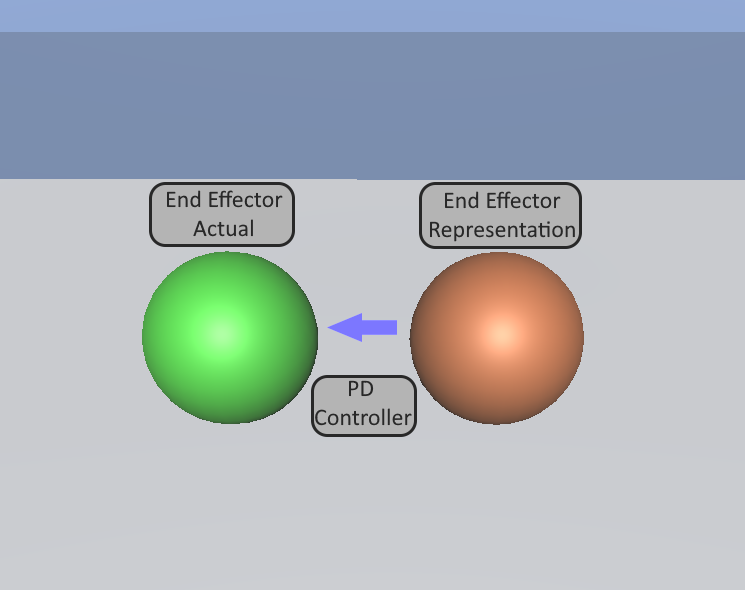
\includegraphics[width=\textwidth]{images/approach-virtual-coupling-a.png}
        \caption{PD controller moves Representation to Actual if there is no obstruction}
        \label{fig:virtual-coupling-a}
    \end{subfigure}
    \quad
    \quad
    \begin{subfigure}[b]{0.4\textwidth}
        \centering
        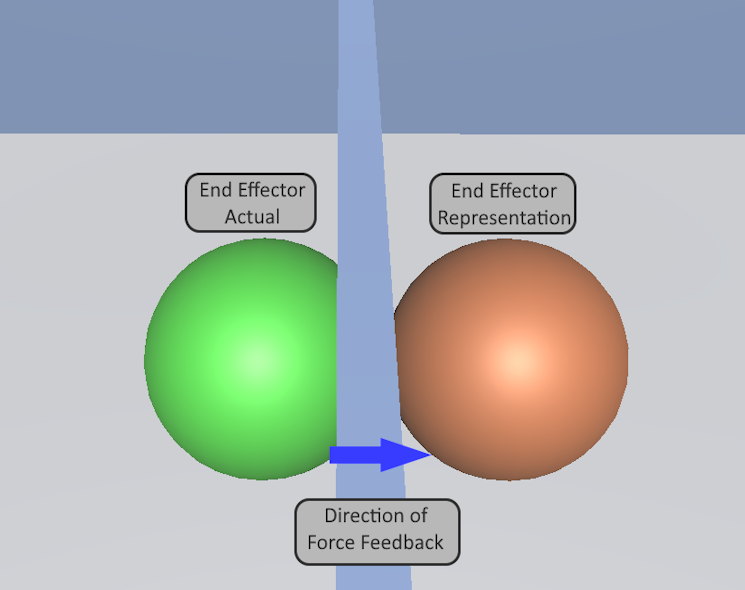
\includegraphics[width=\textwidth]{images/approach-virtual-coupling-b.png}
        \caption{Force Feedback Rendered if physics collision is detected}
        \label{fig:virtual-coupling-b}
    \end{subfigure}
    \caption{Virtual Coupling between Representation and Actual End Effector}
    \label{fig:virtual-coupling}
\end{figure}


\subsection{How would we detect and render textures in realtime?}

Lorem Ipsum

\subsection{How would we design the tool itself, with the main mode of interaction being through the Haply?}

Lorem Ipsum set dolor 


\section{Prototyping} \label{sec:prototyping}
\subsection{Developing for Unity}
There were two main aspects to developing for Unity which we rehaul from the sample Unity Haply Gitlab repository:
\subsubsection{Board Configurations}
Since we have differently configured 2DIY Gen 3 Haply boards (and in some cases, Gen 2 boards), we need a way to switch easily between these configurations without spending time changing code whenever we push code to each other. Given that all the team members in this project worked remotely and in different time zones, this was imperative to a smoother development experience. 

To facilitate this, we change the flow of logic for initialising the board to use configuration files, refered to as scriptable objects in Unity. By storing our different configurations in these files, we can easily swap in the appropriate configuration during development time without affecting any of the actual code.

\begin{figure}
    \centering
    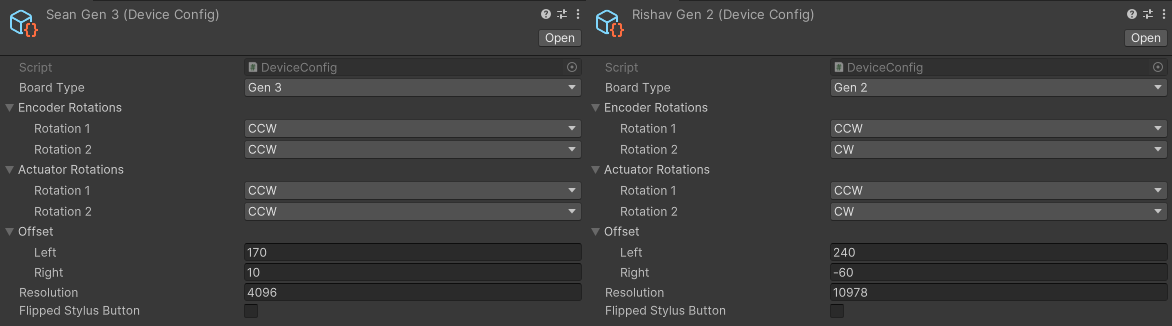
\includegraphics[width = 0.8\textwidth]{images/board-config.png}
    \caption{Different board configurations for the Haply}
    \Description{Different board configurations for the Haply}
    \label{fig:board-config}
\end{figure}

\subsubsection{Utilising Unity's Physics}
The main benefit to utilisng Unity was to leverage it's physics engine for automated haptic experiences. The process of connecting the Haply to Unity physics has been described in detail in \ref{subsec:virtual-coupling}. There are minor nuances in  the implementation itself, specific to Unity. These include making sure the physics engine is running at a higher framerate than normal since the physics is separated from the graphics, enabling continuous collisions for a smoother experience, and interpolating all collisions. While these changes require higher compute, our current application runs at 500+ frames per second, and generally improve the experience without any significant detrmiment to the performanc of the program.

\subsection{Zooming}
In order to allow the designer and user to explore the world at different scales, we incorporate the ability to zoom in and out of the world. From a design perspective, we wished to convey the sense of scale of the world. This was achieved by letting the user explore the ground and the side surfaces of objects in the world when small, and allowing the end effector to "climb" on top of clumps of objects when large, thereby providing force feedback on the basis of the top surface geometry of the objects. 

Implementing this practically was rather trivial, since we had worked extensively on abstracting the texture and object force feedback information. By changing the scale of the representation and moving the camera a proportional amount to said scale, the correct forces and texture data was automatically conveyed. Note that the relationship between the camera's movement and the scaling of the end effector is a cubic one. This is in order to maintain an approximte size of the end effector on screen, such that it gives the appearance of the world growing and shrinking around the designer or the user.

\subsection{Painting}
The incorporation of painting capabilities for objects and textures within a terrain editor is imperative for a multitude of reasons. 
Firstly, such functionality facilitates the creation of intricate and visually captivating landscapes by allowing users to precisely apply diverse textures and objects onto terrain surfaces, thereby enhancing realism and aesthetic appeal. 
More specifically, with the ability to add their own textures and objects, this feature enables users to customize their environments with precision, enabling the realization their artistic visions. 

\begin{figure}[htbp]
    \centering
    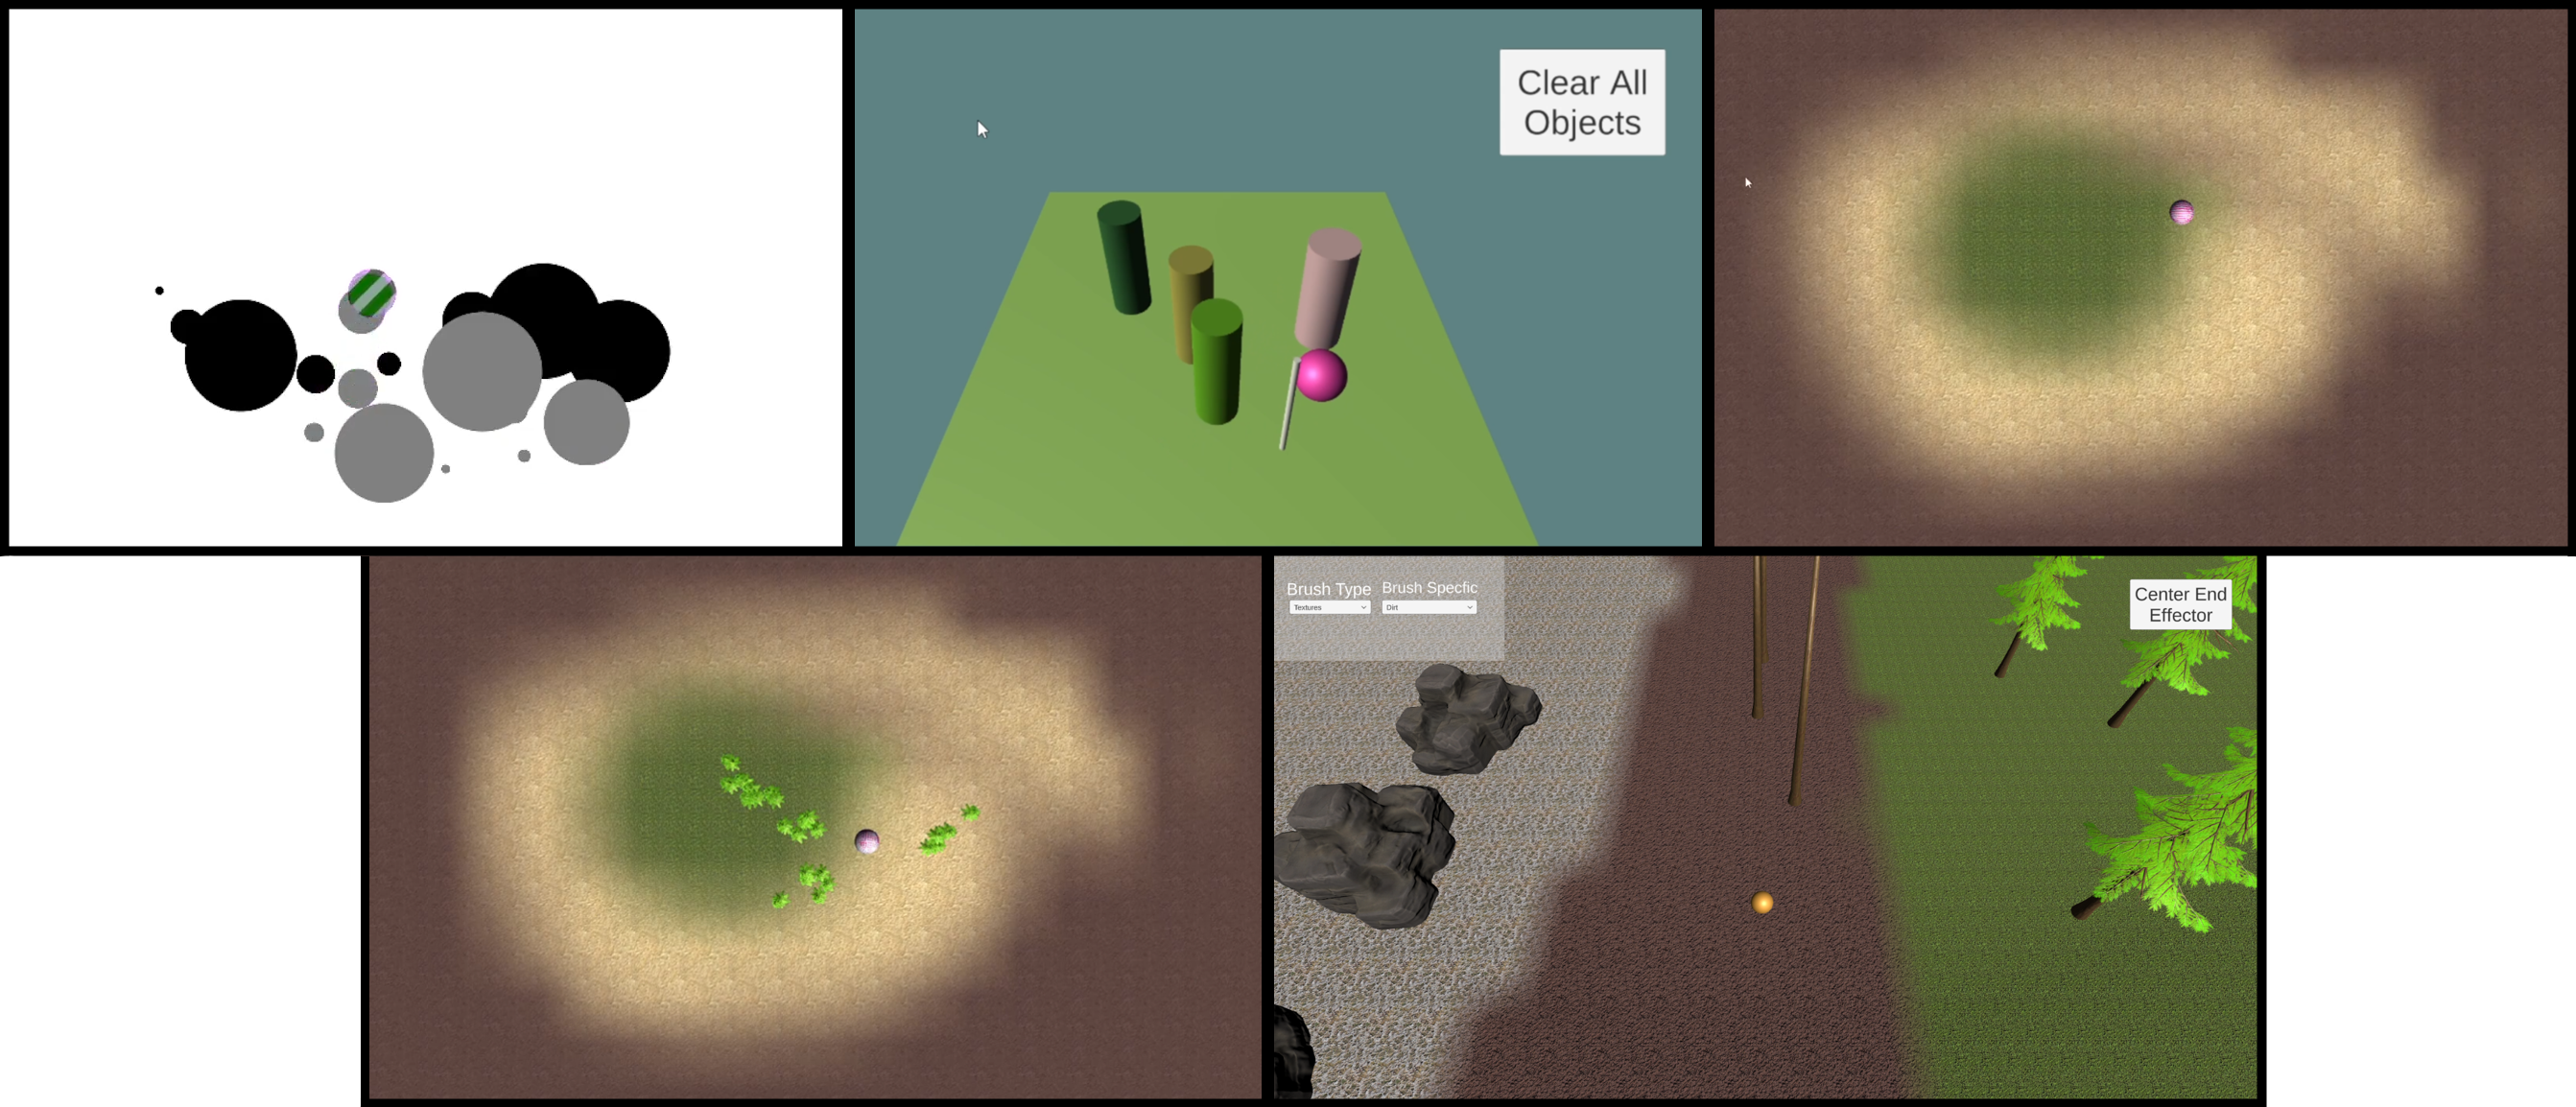
\includegraphics[width=0.8\textwidth]{images/timeline.png} 
    \caption{Representation of the evolution of the prototypes throughout the development of the project
    (1) shows screenshot of the first prototype made to validate our first iteration
    (2) reprensents a screenshot of the first prototype after some code clean up and transfered to 3D space
    (3) displays a screenshot of the texture painting working on Unity's terrain game object
    (4) illustrates painting objects on the the terrain previously textured
    (5) is a capture of the final version which can be seen in Fig. \ref{fig:terrain-painting}}
    \Description{Representation of the evolution of the prototypes throughout the development of the project}
    \label{fig:evolution-painting}
\end{figure}

In line with the comprehensive nature of this project, the process of painting underwent multiple iterations of prototypes throughout the development phase. 
In the forthcoming discussion, we shall examine each prototype and elucidate the insights gleaned from them. 
The creation of our initial prototype, referred to as "the sprinkler," transpired towards the end of the first iteration. 
Its primary objective is to validate the efficacy of the PD controller implementation and the integration of Haply's API for the third iteration of Haply's 2DIY. 
This prototype functioned as a testament to the feasibility of dynamically generating objects during runtime and eliciting force-feedback from interactions between the end-effector and these aforementioned objects.
As illustrated in Figure \ref{fig:texture-rendering}. (1), the sprinkler is placing gray circles as long as we were pressing the stylus button or the spacebar\footnote{the spacebar is used as backup throughout the project if the stylus button doesn't work for diverse reasons}.
These gray circles serve as visual indicators devoid of collision detection, providing a prelude to the subsequent placement of black circles, complete with colliders, upon the eventual release of the stylus button or the spacebar key.


Just after finishing the transition from 2D to 3D, we repurposed the code of "the sprinkler" to be usable in 3D space since it is a quick way to, once again, determine wether or not everything is working as intended.
We are reusing the same logic behind the placement of object as it has proven effective for the first prototype.
In the second image of Figure \ref{fig:texture-rendering}., we can see that the scene is now in 3D and what was previously circles are now cylinders with random colors.
The force-feedback is kept the same, if we move the End-Effector into a cylinder, we will be pushed out as if it is a wall.
We concluded from this prototype that handling the object placement using a similar script is aligned with our goals for object placement, especially since it is easy to use and learn how to use it, thanks to the stylus affordance. 

The subsequent prototype aims to enhance information retention across multiple executions. 
Our approach pivots towards leveraging Unity's terrain game object, which inherently retains terrain deformation, applied textures, and placed objects. 
This strategic alignment enables seamless integration with Unity's terrain editing system, obviating the need for extensive bespoke implementation. 
This not only yields temporal efficiencies but also enhances usability, capitalizing on user familiarity with the platform. 
Our primary focus lies on object and texture painting, thereby excluding terrain elevation adjustments. 

In the prototype corresponding to Figure \ref{fig:texture-rendering}. (3), we introduced the capability to paint textures via mouse input. 
Employing mouse-based prototyping expedites debugging processes, preempting potential issues arising from haptic interfaces. 
This prototype proved its importance in facilitating rapid parameter experimentation, refining aspects such as brush radius, fall-off characteristics, and curve adjustments to ensure smoother edge rendering during texture painting.
From this prototype as a base, we implemented object creation for terrain and object deletion, still utilizing the mouse as an input.
Similarly, it permitted us experiment with different parameters to find what feels best, user experience-wise. 
The results are displayed in Figure \ref{fig:texture-rendering}. (4).

Subsequently, the amalgamation of prototypes culminated in a singular definitive outcome, as depicted in Figure \ref{fig:texture-rendering}. (5).
Firstly, we transitioned the painting process to be contingent upon the positional data of the end-effector representation. 
Secondly, we repurposed the coroutine mechanism utilized for object painting from the second prototype, integrating it seamlessly with newly devised functionalities for object and texture painting, as well as object erasure. 
Lastly, we devised a concise user interface, affording runtime modifications of tools and their respective painting attributes.

\subsection{Texture}
Our initial approach to texture rendering involved firing a raycast to detect the material underneath the end effector. This would then return the corresponding texture information, and the 3x3 window of pixels specifically underneath the end effector representation. Using this we could extrapolate the ideal direction the end effector should be moving. However using raycasts were computationally expensive, and required us to rethink our approach. The texture rendering process in it's current state has been described in detail in \ref{subsec:texture-rendering}, and overall performs better while retaining accuracy in its representation.


\section{Evaluation and Results} \label{sec:evaluation}
Evaluation took the form of a user study, in which we provided a directed walkthrough of our work to novice users, after which we asked a nine linear scale questions about their experience.
We walked users through as follows:

\begin{enumerate}
    \item The user was briefed on the purpose of the project, and that the end effector would be be their point of interaction with the terrain, both for painting and for feedback.
    \item The user was directed through the menu and setup screens.
    \item The user was shown the texture selection menu and told to paint different textures.
    \item The user was allowed to explore this functionality to their satisfaction.
    \item The user was shown the object selection menu and told to paint different objects.
    \item The user was allowed to explore this functionality to their satisfaction.
    \item The user was shown the object deletion menu and told to delete existing objects.
    \item The user was allowed to explore this functionality to their satisfaction.
\end{enumerate}

After this experience, the user was asked the following set of nine 5-point linear scale questions, and told to answer between 5 meaning "most" and 1 meaning "least":
\begin{enumerate}
    \item How easy was it to tell the difference between feedback from objects and feedback from surface textures?
    \item How easy was it to tell the difference between feedback from different surface textures?
    \item How easy was it to tell the difference between feedback from different objects?
    \item How easy was it to tell the difference between feedback from all sources at different zoom levels?
          \vspace{3mm}
    \item How helpful was feedback from objects in understanding and navigating the current state of the terrain?
    \item How helpful was feedback from texture in understanding and navigating the current state of the terrain?
          \vspace{3mm}
    \item How synchronized was haptic feedback with the terrain you saw on screen?
    \item How physically fatiguing did you find the haptic feedback?
    \item How would you rate your overall enjoyment of the experience?
\end{enumerate}

\begin{figure}
    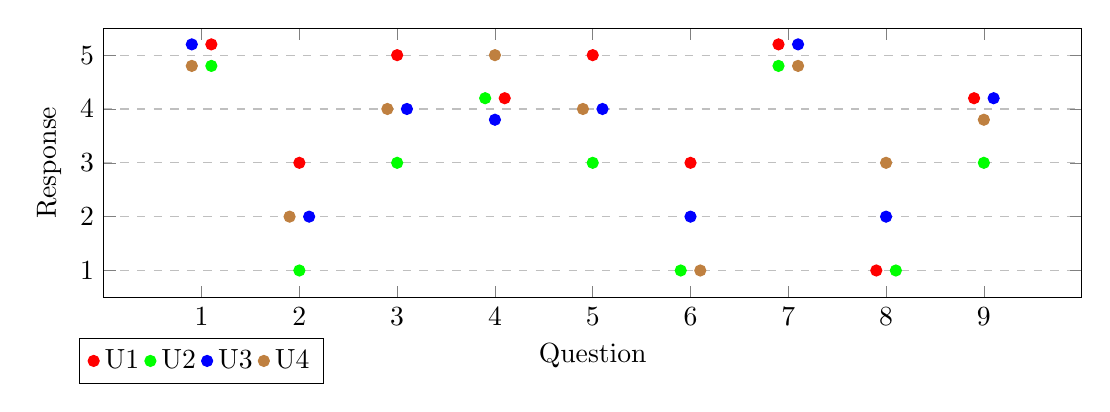
\begin{tikzpicture}
        \begin{axis}[
                width=14cm,
                height=5cm,
                xlabel={Question},
                ylabel={Response},
                xmin=0, xmax=10,
                ymin=0.5, ymax=5.5,
                xtick={1,2,3,4,5,6,7,8,9},
                ytick={1,2,3,4,5},
                legend pos=north west,
                ymajorgrids=true,
                grid style=dashed,
                legend columns=8,
                legend style={at={(0.1,-0.15)},anchor=north}
            ]
            \addplot[only marks, color=red]
            coordinates{(1.1,5.2)(2,3)(3,5)(4.1,4.2)(5,5)(6,3)(6.9,5.2)(7.9,1)(8.9,4.2)};
            \addlegendentry{U1}

            \addplot[only marks, color=green]
            coordinates{(1.1,4.8)(2,1)(3,3)(3.9,4.2)(5,3)(5.9,1)(6.9,4.8)(8.1,1)(9,3)};
            \addlegendentry{U2}

            \addplot[only marks, color=blue]
            coordinates{(0.9,5.2)(2.1,2)(3.1,4)(4,3.8)(5.1,4)(6,2)(7.1,5.2)(8,2)(9.1,4.2)};
            \addlegendentry{U3}

            \addplot[only marks, color=brown]
            coordinates{(0.9,4.8)(1.9,2)(2.9,4)(4,5)(4.9,4)(6.1,1)(7.1,4.8)(8,3)(9,3.8)};
            \addlegendentry{U4}
        \end{axis}
    \end{tikzpicture}
    \caption{User Study Responses}
    \label{fig:user-study}
\end{figure}

The responses to these questions is charted in \autoref{fig:user-study}; we provide data on four respondents, grouped by color. Overall sentiment was positive with respect to force feedback, with all respondents rating both the utility and differentiability of shape-driven feedback highly.
Users generally found it difficult to differentiate between textures, and did not find them helpful for terrain navigation. We conjecture improving texture differentiability would improve the usefulness of this feedback, though in its current state textural feedback still provides users feedback on scale and rate of motion. Users did however find it easy to discriminate scale on the basis of haptic feedback.
Users generally did not find the experience fatiguing, and found it both well-synchronized with the visual terrain rendering and enjoyable overall.

We conclude that users generally felt that feedback from scene objects was both salient and useful, but that textures fell short due to difficulty in differentiation. However, the positive responses for both sentiment, fatigue, and usefulness of shape-driven feedback supports the viability of the project.

\section{Discussions} \label{sec:discussions}
\subsection{Discussions}

\paragraph{The Haptic-Editing process}

Through our evaluation, we discovered that users generally appreciated shape-driven haptic feedback, as it is salient, easily discriminated, offers practical uses like density estimation, and prevents users from overpopulating terrain regions. We also learned that texture feedback as we implement it in this work is of limited usefulness, as many users complained of poor differentiability. Use of a 2D pantograph interface to populate a 2D terrain object was grasped intuitively, and none of our participants had difficulty understanding the connection between the physical end effector and the representation of the end effector in our editor. We claim our interface would be well-suited as a plugin to Unity, allowing game developers to continue using tools they're familiar with, but with the added benefit of haptic feedback for terrain editing and similar applications. Indeed, force and texture feedback are both driven by parts of the engine, colliders and normal maps respectively, that will necessarily be used by a game developer in this context, and thus our interface requires no additional burden to use. 

\paragraph{Unity as a tool for haptics design}

Throughout history, various art forms, such as music, drawing, photography, film, video editing, game development, and XR development, have experienced significant advancements whenever developers have embraced user-friendly tools. These advancements have been facilitated by the availability of accessible cameras, freely available software for music composition and video editing, as well as widely supported game engines like Unity and Unreal. However, when the primary means of entry into these fields is limited to Java and Processing code, the potential for designing experiences becomes constrained by the technical skills of developers, creating a bottleneck effect. It is imperative to encourage the haptics community to explore beyond mere code frameworks and instead adopt a singular, user-friendly engine (such as Unity) that can empower designers to focus on the user experience aspect of haptics, rather than being bogged down by technical jargon. Such an approach would enable individuals to specialize in various aspects of haptics, be it hardware, software, or design, akin to the specialization seen in the game development industry, thereby enhancing the overall quality of output.

\subsection{Limitations}

\paragraph{Movement in an infinite space}

With our current implementation, the end effector can only move in the virtual space a distance proportional to the Haply device's arm length. While we can change the movement scale in the engine, the end effector will eventually get stuck due to the haply's arm pantograph constraint. The primary difficulty lies in changing the relative positioning of the proxy with respect to the world, and what the underlying user experience design philosophy should be for the same without disorienting the user.

\paragraph{Fine grain control of placed objects}
While we have the ability to place objects around a specific space, we do not have the ability to move or rotate a placed object in any degree of freedom, or scale the object up and down. This was an initial consideration our project had but had to be discarded in the interest of time and producing a working prototype. The main issue with this comes in tackling the user interaction model to edit the transform data of an object. Since the haply is the main mode of interaction, we could consider using it similar to a mouse, and designing movement, rotation and scale gizmos that can subsequently be used for the editing process.



\section{Acknowledgments}
 blah blah
\begin{verbatim}
  \begin{acks}
  ...
  \end{acks}
\end{verbatim}


\begin{acks}
To bob.
\end{acks}



\bibliographystyle{ACM-Reference-Format}
\bibliography{refs}
\appendix

\section{Video Figure}

Please find a 2-minute overview of the functionality of our project here:\\ 
\href{https://www.youtube.com/watch?v=PPx2JuhQ9Us}{https://www.youtube.com/watch?v=PPx2JuhQ9Us}

\section{Individual Contributions}

\subsection{Rishav's Contributions}

\begin{figure}[htp]
    \centering
    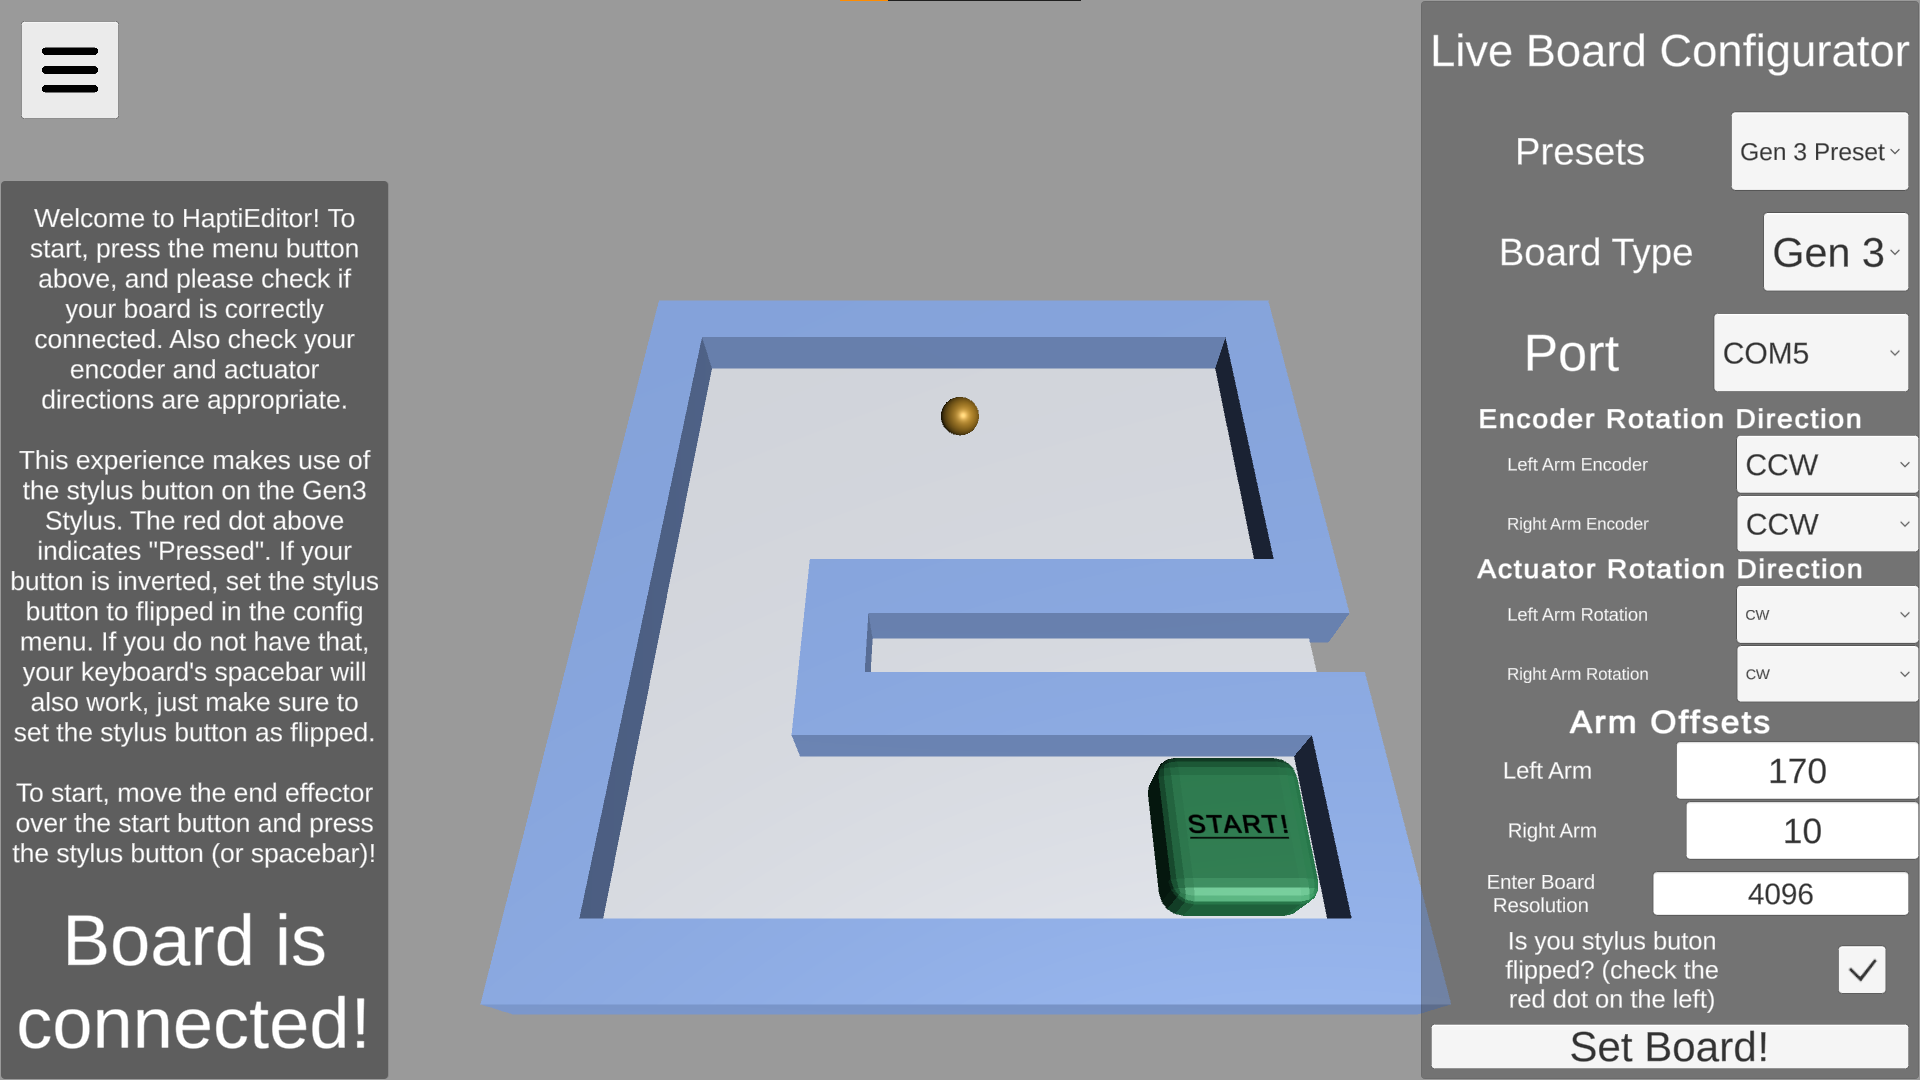
\includegraphics[width=14cm]{images/appendix-menu.png}
    \caption{HaptiEditor configuration menu}
    \Description{HaptiEditor configuration menu}
    \label{fig:menu}
\end{figure}

For the final iteration, we wanted to build an executable that anyone with a haply 2diy board can plug and play. Expecting everyone to install Unity would be quite an ask, so we needed to build a live board configurator.

The live board configurator would need to modify the following parameters:
\begin{itemize}
    \item Board Presets
    \item Gen2 or Gen3 (for arm distance offset)
    \item Encoder rotation direction
    \item Actuator rotation direction
    \item Arm offsets for base position
    \item Encoder resolution
    \item Flipped Stylus Button (Some Gen3 boards have flipped sensor data for the stylus port)
\end{itemize}

Actually passing the appropriate data and reloading the board was significantly more difficult. In a nutshell, I had to do the following:
\begin{itemize}
    \item Cancel the worker thread simulation task gracefully
    \item Flush all forces
    \item Delete the existing instance of the board (along with the encoder, actuator and sensor parameters)
    \item Create a new board instance with the new parameters
    \item Attempt a connection to the new specified port based on the user’s selection from current active ports
    \item Launch a new worker thread.
    \item Potentially connect to a Button Handler if the scene had one present.
\end{itemize}

This required a significant amount of refactoring of the core hAPI, but in the end I was successfully able to load and reload new user specified board configurations. The main chunk of this was happening in the \texttt{EndEffectorManager.cs} as follows:

\begin{minted}[style=friendly, linenos,fontsize=\footnotesize]{csharp}
public void ReloadBoard(DeviceConfig customConfig, string targetPort)
{
    // Destroying existing setup
    haplyBoard.DestroyBoard(); // added function to close port and destroy this board
    CancelSimulation();
    SetForces(0f, 0f);
    Destroy(pantograph.gameObject.GetComponent<Device>());
    // New Setup
    device = pantograph.gameObject.AddComponent<Device>();
    device.Init(); // re-establishes basic connections with pantograph and board
    LoadBoard(customConfig, targetPort);
    // Checking for button handler
    ButtonHandler buttonHandler = gameObject.GetComponent<ButtonHandler>();
    if (buttonHandler == null) return;
    buttonHandler.SetButtonState(customConfig.FlippedStylusButton);
}

private void LoadBoard(DeviceConfig customConfig = null, string targetPort = null)
{
    device.LoadConfig(customConfig);   // loads new config if custom config is not null
    haplyBoard.Initialize(targetPort); // attempts connection with new port
    device.DeviceSetParameters();
    // ...
    simulationLoopTask = new Task( SimulationLoop );
    simulationLoopTask.Start();
}
\end{minted}

After this, I decided to improve the visual experience of the project. Users will be expected to understand that they have to configure their board, and that their board might be set up different to our dev setups, so the menu scene should ideally be different from the actual terrain editing scene. Additionally, the stylus button (or space bar) is critical to the experience, so the users should be aware of how to do that as well.

To let the user learn this separately, I worked on a simple menu scene with a bit of flair, and added scene transitions. Users will now be expected to first configure their board, be able to move over a physical button in the world, and then click on the stylus button to enter the terrain painter tool.

I fished out a basic scene manager and transition handler from an older project, and after some tweaking, blender modelling and building an executable for Windows, I produced the menu scene in \autoref{fig:menu}.

\subsection{Sean's Contributions}

This iteration, I finalized work on the texture pipeline and integrated it with Pierre’s work from iteration 2 on texture and object painting on the terrain object. Pierre wrote some logic to get world position into a corresponding position on the surface of the terrain object, removing the need for our expensive physics ray-cast. The rest of the process involved the following changes:

\begin{itemize}
    \item Detecting which terrain texture was currently painted onto the surface of the terrain underneath the end effector. This required fetching the blend ratios of each material at the EE location and determining which was present:

          \begin{minted}[style=friendly, linenos,fontsize=\footnotesize]{csharp}
float[,,] swatch = terrain.terrainData.GetAlphamaps((int)pixelUV.x, (int)pixelUV.y, 1,1);
\end{minted}

    \item Once I have the ID of the texture to sample, we fetch color from its normal texture, giving us both a direction and intensity of force we immediately apply to our end effector. This greatly simplified the sampling code:

          \begin{minted}[style=friendly, linenos,fontsize=\footnotesize]{csharp}
Color normalPixel = prot.normalMap.GetPixel((int)normalUV.x, (int)normalUV.y);

forces.x += normalPixel.r - 0.5f
forces.y += normalPixel.g - 0.5f;

forces *= intensity;
previousPosition = eeTransform.position;
\end{minted}

    \item  I introduced a variable \texttt{swatchscale} to allow us to control the ratio of world movement relative to movement on the normal map, controlling the linear density of our texture. Normal sampling also greatly improved the accuracy of forces, as we’re no longer estimating heightmaps from surface color but now have geometry-accurate normal maps.
    \item  Selected texturally distinct normal maps for our materials for a clearer distinction between painted materials.
    \item  Added back space-bar support for painting, so a user has an alternative to the stylus button.
\end{itemize}

I then tuned the scaling code Rishav worked on in iteration 2 and added it to our scene. The following changed:

\begin{itemize}
    \item I added a scale factor for the movement range of the end effector, so it expanded as the scene zoomed out, covering the new area.
    \item I then tuned the ratios for movement range, end effector size and camera zooming so that they scaled in tandem.
    \item I changed the painter code so that the painted objects had their appropriate colliders, allowing the large end effector to skate over rocks as we’d intended it to, rather than getting stuck like before.
\end{itemize}

Lastly, I tuned the texture sampling code again so that it would play nice with the zooming feature we’d introduced. I chose a \texttt{swatchscale} such that at high zoom levels, individual surface features like pebbles were quite large and discernible, but with a wider camera, surface features became higher frequency noise and force feedback from geometry became the primary force on the end effector. Textures representations were different depending on the painted texture on the terrain and could be rendered in tandem with terrain objects placed during use. We learned that these pipelines could all coexist in a cohesive way and were pleased to see our parallel approach to developing them paid off.

Post iteration 3, I fixed some outstanding bugs, worked on my section of the report, and prepared the video figure.

\subsection{Pierre's Contributions}
As stated in our blog posts for iteration 2, the goal for the third was to merge every concepts and prototypes into one single, preferably enjoyable, experience. In this iteration we ended up working together way more and in closer collaboration by helping each others a lot more. This can be easily explained because we didn’t prototype on a different aspect of the experience and were actually making something unique together. This is why sometimes the lines of contributions of what I did and what a team member did will blur into what we did this feature together.

While we knew that we would merge all of our progress into the Terrain scene because the end goal is to use Unity’s Terrain game object has our editor, the \texttt{TerrainScript.cs} from iteration 2 wasn’t usable as is. Firstly, we need to fix the lack optimizations. Secondly, the user should have a way to change the brush type and their specifics without using Unity editor menus (it is necessary if the user interacts with our software through an executable instead of the Unity Project). Thirdly, Lastly, it is unlikely the code we used for texture sampling for haptic feedback would work on the Terrain game object, because it has the particularity to not have a \texttt{MeshRenderer} (a component that allows a game object to render a mesh). Finally, there needs to be a way paint using the stylus button instead of the mouse.

During this iteration Rishav did an amazing work at going over the code that has been made and telling us what should be avoided in the future. Following those practices we started a refactoring on \texttt{TerrainScript.cs}.  During this time, I found a way to optimize the management of the \texttt{TreeInstances} what were giving us issues during the second iteration, basically, deleted \texttt{TreeInstances} would never really be deleted but replaced with empty version of themselves.

This is problematic because with the core logic of the problem they would be given another collider the next time the software is running even though there is nothing to delete.

\begin{minted}[style=friendly, linenos,fontsize=\footnotesize]{csharp}
private void OnApplicationQuit()
{
    //test
    List<TreeInstance> trees = new List<TreeInstance>(terrain.terrainData.treeInstances);
    List<TreeInstance> trees_cleaned = new List<TreeInstance>();
    TreeInstance empty_tree = new TreeInstance();
    for (int i = 0; i < trees.Count; i++)
    {
        if (!trees[i].Equals(empty_tree))
            trees_cleaned.Add(trees[i]);
    }
    terrain.terrainData.SetTreeInstances(trees_cleaned.ToArray(), true);
}
\end{minted}

Using this code when the application is closed we remove all of the \texttt{TreeInstances} that we could consider empty. The way it works is by going through all the objects in the Terrain \texttt{TreeInstances}  and comparing it with an empty object. If they are different we add them to the new list that will contain all the non-empty \texttt{TreeInstance}.

Then using the \texttt{ObjectPlacer.cs} as a reference I created two co-routines one for painting object on the terrain and the other for painting texture. We implemented an enumerator containing all the brushes types (i.e. Texture, Object and Object Eraser) and depending on this brush type one of the co-routine or the object deletion will be enabled.

From then on Rishav worked with me on a basic UI so we can change the brush types and which texture/object is being painted.

\subsection{Previous Iterations}

\end{document}
\endinput
%%
%% End of file `sample-manuscript.tex'.
